% !TeX root = ../main.tex

\chapter{系统测试与分析}
前面的章节介绍了系统的需求分析和设计实现,本章将对系统的功能性需求和非功能性需求进行测试,重点阐述测试方法和测试环境,给出相应的测试结果,并根据测试结果做对应的分析。

本次测试主要分为三个模块,分别是持续性测试、性能测试和对比测试。在持续性测试中,测试环境会模拟用户对系统的操作,持续地调用系统的接口,我们可以通过观察调用接口的结果来判定系统是否能够实现预期的功能,也能够对非功能性需求中的可用性、可扩展性和安全性进行验证。性能测试主要是用来验证系统的性能是否符合预期,测试的方法是将系统部署之后,用户在不同区域通过网络访问系统,测试结果受制于用户的网络状态和机器性能。通过性能测试,可以验证我们的系统是否是否完成了非功能性需求中对性能的要求。

除此之外,本章还进行了对比测试与分析,将本系统和其他同类产品进行了对比测试或分析,通过测试数据和理论分析证明我们的系统在某些方面具有优势。

\section{持续性测试}%6.1
\subsection{测试方法}%6.1.1
由于系统在不断地迭代更新,简单的基于API的测试让测试本身限于被动且不具备可持续性,不能满足测试要求,从用户角度来说,无论系统的服务如何改造,其核心诉求仍然不变,即无论何时,对外的功能不能改变,没有被删除的文件应总能下载,且数据完整性不会被破坏。基于此,我们设计了一个专为验收的测试环境,在这个环境中会模拟用户请求对系统发起访问,系统需要长期在测试环境运行。验收时,主要观察接口的响应结果,验证结果是否符合预期,是否满足功能性需求。除此之外,持续性测试也需要验证系统的相关非功能性需求,即系统在各种异常情况下能否维护数据一致性,磁盘和服务级别的故障是否会影响上传下载等相关业务。为此,环境会模拟机器损坏,随机将某单一服务停止运行一段时间,然后将其进行重启,还会模拟磁盘故障,使磁盘数据出错。
\subsection{测试环境}%6.1.2
系统是一个分布式系统,在测试时需要将各个服务在各节点上分开服务,这些节点同在一个局域网内可以进行通信,我们准备了两种服务器来进行测试。
第一种服务器用来部署storage服务,它的具体参数如表6.1所示。

\begin{table}[h]
    \centering
    \caption{服务器A参数表}
    \begin{tabular}{cc}
      \toprule
      项目   & 配置参数   \\
      \midrule
      网卡带宽  & 10Gb*2  \\
      CPU核数   & 48C     \\
      Memory   & 64G      \\
      SATA     & 8T *23   \\
      \bottomrule
    \end{tabular}
\end{table}

第一种服务器用来部署除storage以外的服务,它的具体参数如表6.2所示。

\begin{table}[h]
    \centering
    \caption{服务器B参数表}
    \begin{tabular}{cc}
      \toprule
      项目   & 配置参数   \\
      \midrule
      网卡带宽  & 10Gb*2  \\
      CPU核数   & 48C     \\
      Memory   & 64G      \\
      \bottomrule
    \end{tabular}
\end{table}

本次测试的系统中块大小为16MB,使用R=2,N=4,M=2的配置来设置系统,即每个条带有两个副本,每个条带数据块有4块,EC校验块有2块。

由于系统不是单独调用每个接口来进行测试,而是将系统部署在测试环境中进行运行,因此在这里我们需要定义测试环境中如何模拟用户的请求。与此同时,测试环境还需要模拟系统中出现各种故障,所以还需要定义需要常态化模拟的故障场景。测试环境内需要进行的工作主要如下:

1. 服务将会随机异常重启

这里主要是对storage服务进行随机异常停止。storage停止服务意味着单点故障,发生单点故障时可以利用条带的冗余策略读取副本或者利用EC校验块恢复数据,加入这类故障可以检测系统能否提供一定的可用性。

2. 磁盘损坏测试

磁盘损坏在系统正式运行时并不是一件极其罕见的事,在测试环境中需要模拟这种情况。测试环境中主要模拟磁盘数据损坏的情况,随机地将磁盘中的数据进行更改。系统不能因为磁盘数据的损坏而返回错误的结果,需要利用磁盘中的循环冗余校验码的值来检测这种情况,防止将错误数据返回。

3. 进行系统扩容

在测试过程中,系统的容量不应保持恒定,应该引入扩容操作来测试系统是否具有良好的可扩展性,扩容时应观察系统是否能正常提供服务。

4. 记录接口的调用情况

测试环境需要记录模拟用户调用的请求的具体情况,包括请求的地址和参数、响应结果、接口调用时间等信息。测试的结果将通过观察这些请求,分析系统是否按期望返回正确的结果。

\subsection{测试内容与计划}%6.1.4
为了测试功能性需求,在测试环境加入了以下的测试用例。

1. 用户数据操作测试

如表6.3所示,在测试环境中会模拟用户进行以下的用户数据管理操作。

\begin{table}[h]
  \centering
  \caption{用户数据操作用例表}
  \begin{tabular}{cc}
    \toprule
    模拟的操作   & 预期结果   \\
    \midrule
    创建重名用户           & 返回错误,提示重名  \\
    未鉴权修改用户信息     & 返回错误,提示未鉴权     \\
    未鉴权查看用户信息     & 返回错误,提示未鉴权  \\
    创建非重名用户         & 操作合法,修改用户     \\
    鉴权后修改用户信息     & 操作合法,修改用户信息     \\
    鉴权后查看用户信息      & 操作合法,返回用户信息     \\
    \bottomrule
  \end{tabular}
\end{table}

2. 桶数据操作

如表6.4所示,在测试环境中会模拟用户进行以下的桶数据管理操作。

\begin{table}[h]
  \centering
  \caption{桶数据操作用例表}
  \begin{tabular}{cc}
    \toprule
    模拟的操作   & 预期结果   \\
    \midrule
    创建重名桶           & 返回错误,提示重名  \\
    删除不属于自己的桶    & 返回错误,提示桶归属错误     \\
    修改不属于自己的桶    & 返回错误,提示桶归属错误  \\
    修改后桶出现重名      & 返回错误,提示重名  \\
    查看不属于自己的桶    & 返回错误,提示桶归属错误     \\
    创建非重名桶          & 操作合法,创建桶  \\
    删除属于自己的桶      & 操作合法,删除桶     \\
    修改自己的桶且不重名   & 操作合法,修改桶信息  \\
    查看自己的桶          & 操作合法,返回桶信息     \\
    查看自己创建的全部桶   & 操作合法,返回创建的桶信息     \\
    \bottomrule
  \end{tabular}
\end{table}

3. 文件管理操作

如表6.5所示,在测试环境中会模拟用户进行以下的文件管理操作。

\begin{table}[h]
  \centering
  \caption{文件管理操作用例表}
  \begin{tabular}{cc}
    \toprule
    模拟的操作   & 预期结果   \\
    \midrule
    重命名不属于自己的文件     & 返回错误,提示文件归属错误  \\
    重命名文件后重名          & 返回错误,提示重名     \\
    移动不属于自己的文件       & 返回错误,提示文件归属错误  \\
    移动文件后重名            & 返回错误,提示重名  \\
    查看不属于自己的文件信息   & 返回错误,提示文件归属错误     \\
    重命名自己的文件且不重名   & 操作合法,重命名文件  \\
    移动自己的文件且不重名     & 操作合法,移动文件     \\
    查看自己的文件信息        & 操作合法,返回文件信息  \\
    查看桶内全部文件          & 操作合法,返回桶内文件信息     \\
    \bottomrule
  \end{tabular}
\end{table}

4. 文件交互操作

如表6.6所示,在测试环境中会模拟用户进行以下的文件交互操作。
\newline

\begin{table}[h]
  \centering
  \caption{文件交互操作用例表}
  \begin{tabular}{cc}
    \toprule
    模拟的操作   & 预期结果   \\
    \midrule
    上传文件至无上传权限的桶   & 返回错误,提示没有权限  \\
    下载没有下载权限的文件     & 返回错误,提示没有权限  \\
    删除不属于自己的文件       & 返回错误,提示文件归属错误  \\
    下载不存在的文件          & 返回错误,提示找不到文件  \\
    上传文件至有上传权限的桶   & 操作合法,文件上传成功  \\
    下载有权限下载的文件       & 操作合法,返回文件数据  \\
    删除自己的文件            & 操作合法,删除对应文件  \\
    \bottomrule
  \end{tabular}
\end{table}

测试环境在模拟用户操作时会对系统进行循序渐进的测试,开始时不会令系统发生异常,所有接口调用都是常规操作,后续会引入系统异常,检测在异常状态下是否能够正确提供服务,具体的测试计划如表6.7所示。

\begin{table}[h]
    \centering
    \caption{测试计划表}
    \begin{tabular}{cc}
      \toprule
      环境状况   & 时间   \\
      \midrule
      无异常,只开启随机扩容  & 7天  \\
      引入异常,随机停止服务  & 3天     \\
      模拟磁盘损坏           & 3天  \\
      以上三种并行           & 4天     \\
      \bottomrule
    \end{tabular}
\end{table}

\subsection{测试结果与分析}%6.1.5

经过测试之后,我们需要观察接口的调用情况,分析系统是否能满足功能性需求,经过观察后,得出下面的测试结果和相关分析。

1. 桶数据管理操作

桶数据操作的测试结果如表6.8所示。

\begin{table}[h]
  \centering
  \caption{桶数据操作测试结果表}
  \begin{tabular}{cc}
    \toprule
    模拟的操作   & 测试结果   \\
    \midrule
    创建重名桶           & 提示重名,符合预期  \\
    删除不属于自己的桶    & 提示桶归属错误 ,符合预期    \\
    修改不属于自己的桶    & 提示桶归属错误,符合预期  \\
    修改后桶出现重名      & 提示重名,符合预期  \\
    查看不属于自己的桶    & 提示桶归属错误,符合预期     \\
    创建非重名桶          & 创建桶,符合预期  \\
    删除属于自己的桶      & 删除桶,符合预期     \\
    修改自己的桶且不重名   & 修改桶信息,符合预期  \\
    查看自己的桶          & 返回桶信息,符合预期     \\
    查看自己创建的全部桶   & 返回创建的桶信息,符合预期     \\
    \bottomrule
  \end{tabular}
\end{table}

以上测试结果表明,系统能较好地完成文件交互操作的功能性需求。

2. 用户数据管理操作测试结果

用户数据管理操作的测试结果如表6.9所示。测试结果表明,系统能较好地完成文件交互操作的功能性需求。
\newline

\begin{table}[h]
  \centering
  \caption{用户数据操测试结果表}
  \begin{tabular}{cc}
    \toprule
    模拟的操作   & 测试结果   \\
    \midrule
    创建重名用户           & 提示重名,符合预期  \\
    未鉴权修改用户信息     & 提示未鉴权,符合预期     \\
    未鉴权查看用户信息     & 提示未鉴权,符合预期 \\
    创建非重名用户         & 修改用户,符合预期    \\
    鉴权后修改用户信息     & 修改用户信息,符合预期    \\
    鉴权后查看用户信息      & 返回用户信息,符合预期   \\
    \bottomrule
  \end{tabular}
\end{table}

3. 文件管理操作

文件管理操作的测试结果如表6.10所示。

\begin{table}[h]
  \centering
  \caption{文件管理操作测试结果表}
  \begin{tabular}{cc}
    \toprule
    模拟的操作   & 测试结果   \\
    \midrule
    重命名不属于自己的文件     & 提示文件归属错误,符合预期  \\
    重命名文件后重名          & 提示重名,符合预期     \\
    移动不属于自己的文件       & 提示文件归属错误,符合预期  \\
    移动文件后重名            & 提示重名,符合预期  \\
    查看不属于自己的文件信息   & 提示文件归属错误,符合预期     \\
    重命名自己的文件且不重名   & 重命名文件,符合预期  \\
    移动自己的文件且不重名     & 移动文件,符合预期     \\
    查看自己的文件信息        & 返回文件信息,符合预期  \\
    查看桶内全部文件          & 返回桶内文件信息,符合预期     \\
    \bottomrule
  \end{tabular}
\end{table}

以上测试结果表明,系统能较好地完成文件交互操作的功能性需求。

4. 文件交互操作

文件交互操作的测试结果如表6.11所示。

\begin{table}[h]
  \centering
  \caption{文件交互操作测试结果表}
  \begin{tabular}{cc}
    \toprule
    模拟的操作   & 测试结果   \\
    \midrule
    上传文件至无上传权限的桶   & 提示没有权限,符合预期  \\
    下载没有下载权限的文件     & 提示没有权限,符合预期  \\
    删除不属于自己的文件       & 提示文件归属错误,符合预期  \\
    下载不存在的文件          & 提示找不到文件,符合预期  \\
    上传文件至有上传权限的桶   & 文件上传成功,符合预期  \\
    下载有权限下载的文件       & 返回文件数据,符合预期  \\
    删除自己的文件            & 删除对应文件,符合预期  \\
    \bottomrule
  \end{tabular}
\end{table}

以上测试结果表明,系统能较好地完成文件交互操作的功能性需求。

通过以上的结果,我们分析得出系统能较好地实现功能性需求,接下来我们分析系统是否满足了非功能性需求。

在测试环境中,不仅模拟了正确的操作,还模拟了一些在没有权限的情况下访问系统的情况,例如下载未授权下载的文件和删除不属于自己的文件等,在我们的测试中,系统拒绝了这些访问,并返回鉴权失败,证明系统能够满足安全性的要求。

在测试计划中,阐述了系统在进行持续测试时会进行随机扩容的操作,经观察,系统不会因为扩容操作而影响业务操作,证明系统具有一定的可扩展性。

在测试计划中,阐述了系统在进行测试时会引入服务重启和磁盘故障,我们可以通过观察接口的响应时间和下载的数据是否出现错误来判断系统是否具有一定的可用性如果响应时间过长意味着系统的接口出现了超时,也就是出现了不可用的情况。经观察,系统不会因为某个服务的中断或单个磁盘的故障而出现超时或数据出错的现象,这意味着在测试时间内,系统没有出现不可用的情况,说明系统具有一定的可用性。

需要注意的是,以上的结果都是在测试时间内系统运行的结果,在测试时间内没有出现异常不代表系统永远不会出现异常,尤其对于可用性这项指标而言,只有当系统运行的时间达到一定期限后,统计它们的数字才有意义,系统在后续的迭代开发中也会持续使用测试环境进行观察,及时发现系统的异常。

\section{性能测试}%6.2
性能测试的主要目的是使用户了解系统在实际使用时普遍具有的性能,测试时使用指定测速区域部署的系统,向该区域的系统中上传大小为100MB的文件来进行网络测速。这样的测试更贴近用户的实际体验,用户可以到线上的web环境中手动测试,可以得到如图6.1的结果。

\begin{figure}
    \centering
    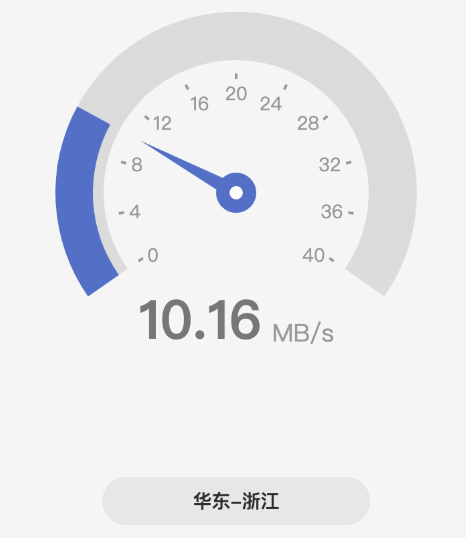
\includegraphics[width=0.33\textwidth]{常规测试结果图.png}
    \caption{常规测试结果图}
\end{figure}

本次测试将测试多个位置部署的系统,测试的客户端位置位于上海,测试结果如表6.12所示。

\begin{table}[h]
    \centering
    \caption{多位置测试结果表}
    \begin{tabular}{cc}
      \toprule
      系统部署位置   & 速度(MB/s)   \\
      \midrule
      华东-浙江     & 10.16  \\
      华北-河北     & 8.15   \\
      华南-广东     & 8.42  \\
      亚太-新加坡   & 4.3   \\
      北美-洛杉矶   & 5.08  \\
      \bottomrule
    \end{tabular}
\end{table}

可以看到用户上传的速度主要取决于网络情况,访问物理链路较长的系统速度较慢。

\section{对比测试与分析}%6.3
以上两个小节的测试主要是为了测试系统是否满足了功能性需求和非功能性需求。本小节将进行对比测试,主要目的是和同类型产品进行对比,通过测试或分析后,检验我们设计的系统是否与其他产品在某些方面具有优势。

\subsection{和Haystack对比}%6.3.1
在1.2.1章节中,我们介绍了Facebook开发的分布式对象存储系统Haystack,它以多副本的方式来实现系统的容错,并没有采用纠删码来对文件进行冗余。相较于这类只使用多副本而没有使用纠删码进行容错的系统,我们系统的优势是存储的成本更低,配置更加灵活。纠删码支持k+r种任意组合,k指的是数据块的数量,r指的是校验数据的数量。以28+4的纠删码为例,磁盘的利用率为k/(k+r),即28/32=73.7%,而三副本的磁盘利用率为33%,我们的系统在磁盘利用率上有较大的优势。除此之外,我们的系统可以根据自己的需求更灵活地进行配置,通过控制k和r的值来达到所需的效果。k值影响数据恢复代价,k值越小,数据分散度越小,故障影响面越大,但恢复代价低;k值越大,数据分散度则越大,故障影响面越小,但重建代价也越大。r值影响容错能力与存储成本,r值越大,故障容忍度越高,存储效率越低;r值越小,故障容忍度越低,存储效率越高。一般情况下,纠删码使数据更加分散,容错性更好,以28+4的纠删码为例,可以在4个节点损坏时保证的数据正常访问,而三副本最多只能同时损坏2个节点。

相对应的,相比之下,我们系统的缺陷是恢复成本较大。在进行错误恢复时,多副本系统只需读取副本数据即可,而纠删码系统需要将冗余的数据块全部读取后再进行计算,导致数据在纠删码状态下有故障读时性能更差。为了应对这个缺陷,我们可以控制EC策略,当条带内数据冷却后再转换为纠删码存储,尽可能减少纠删码条带的读取。

\subsection{和MinIO对比}%6.3.2
在2.2.3章节中,我们详细介绍过MinIO这款分布式对象存储系统,它使用纠删组的形式组织文件,文件都以纠删码的形式存放在系统中。在设计分析章节,我们分析过使用纠删码时小文件写入性能较差,因此相较于这种只使用纠删码的系统,我们系统的优势是在大量小文件存储场景下性能有优势。

为了比较两者在大量小文件场景下的性能,我们搭建了以下的测试环境对性能进行测试。环境中共有16个节点,每个节点的配置如表6.13所示,每个节点中配置了4*1TB的磁盘,其中8个节点作服务端,8个节点作客户端。

\begin{table}[h]
    \centering
    \caption{节点参数表}
    \begin{tabular}{cc}
      \toprule
      项目   & 配置参数   \\
      \midrule
      网卡带宽 & 10Gb*2  \\
      CPU核数  & 48C     \\
      Memory  & 64G      \\
      SSD     & 1T *4   \\
      \bottomrule
    \end{tabular}
\end{table}

首先测试MinIO的性能,客户端开启32线程测试1M大小的文件上传下载性能,持续时间30秒,得到结果如表6.14所示。

\begin{table}[h]
    \centering
    \caption{MinIO测试结果}
    \begin{tabular}{ccc}
      \toprule
      客户机   & PUT吞吐量  & GET吞吐量 \\
      \midrule
      节点1  & 62.2MB/s  & 316.7MB/s \\
      节点2  & 62.1MB/s  & 320.3MB/s \\
      节点3  & 62.5MB/s  & 317.3MB/s \\
      节点4  & 62.4MB/s  & 319.2MB/s \\
      节点5  & 62MB/s    & 319.3MB/s \\
      节点6  & 62.5MB/s  & 300.6MB/s \\
      节点7  & 62.4MB/s  & 318.5MB/s \\
      节点8  & 62.6MB/s  & 319.5MB/s \\
      汇总   & 498.7MB/s & 2531.4MB/s \\
      \bottomrule
    \end{tabular}
\end{table}

使用同样的测试参数,测试我们开发的系统,得到的结果如表6.15所示。

\begin{table}[h]
    \centering
    \caption{本系统测试结果}
    \begin{tabular}{ccc}
      \toprule
      客户机   & PUT吞吐量  & GET吞吐量 \\
      \midrule
      节点1  & 85.8MB/s  & 320.8MB/s \\
      节点2  & 88.7MB/s  & 319.7MB/s \\
      节点3  & 79.9MB/s  & 328.5MB/s \\
      节点4  & 89.2MB/s  & 318.2MB/s \\
      节点5  & 90MB/s    & 327.7MB/s \\
      节点6  & 86.4MB/s  & 300.8MB/s \\
      节点7  & 79.4MB/s  & 327.6MB/s \\
      节点8  & 88.6MB/s  & 322.4MB/s \\
      汇总   & 688MB/s   & 2567.7MB/s \\
      \bottomrule
    \end{tabular}
\end{table}

从以上的测试结果来看,MinIO和本系统在小文件读取性能上大致相似,在小文件写入性能上本系统有一定优势。原因是测试过程不考虑故障读,所有读取都能够成功返回,无需使用纠删码进行数据的恢复,性能差距不大,而写入时本系统优先写入三副本系统,无需额外计算纠删码,而MinIO使用纠删码写入,需要计算出纠删码后再写入系统,同时MinIO需要将小文件进一步切分,在文件系统中写入时有一定的写放大的问题。

\subsection{和NOS对比}%6.3.3
在2.2.4章节中,我们介绍了网易开发的NOS分布式对象存储系统,它使用多副本和纠删码结合的方法来保存文件,在文件从多副本转为纠删码时,NOS通过LifeCycle程序将文件转入EC池。相较于这类系统,我们系统的最大优势是在文件从多副本到纠删码转换时不需要额外的操作,文件的多副本形式和纠删码形式都是以条带保存在系统中,在保存形式发生改变时,不需要进行额外的存取,避免了文件的多次读写,减少了系统的读写开销。

由于NOS是网易提供的对象储存的云服务,我们无法在同一环境下进行对比测试,因此这里使用实习所在公司的数据,计算使用本系统带来的优化。根据实习所在公司的统计,绝大多数的业务不会频繁删除写入系统的数据,只有约10$\%$的数据将在多副本存储阶段删除,约90$\%$的数据需要由多副本存储系统迁移至纠删码存储系统。也就是说,每写入100MB的文件,将会有90MB的数据需要进行系统级的迁移,迁移过程中不仅需要额外将这些数据写入纠删码系统,而且还需要在纠删码系统保存这些数据的元数据信息,这些工作相较于我们设计的系统而言属于额外写入开销。根据迁移策略的不同,对纠删码存储系统造成的影响也不同,如果用大批量迁移的策略,等多副本系统的使用量满足一个较大阈值时进行迁移,那么将会有大量数据同时写入纠删码系统,造成网络和IO资源的挤占,影响其他业务;如果采用小批量迁移的策略,多副本系统中每完成若干条带的写入后就进行迁移,文件则会频繁写入纠删码系统的存储器,消耗系统性能。

\section{本章小结}%6.4
本章主要对该应用做了全面的测试,搭建了一个测试环境,在该环境中能动态地模拟线上实际操作,通过观察系统是否做出正确响应来验证功能性需求。在验证系统性能时,考虑了用户所处的物理位置和机器性能,验证了系统部署后的实际性能表现。本章还进行了对比测试与分析,通过测试数据和理论分析证明我们设计的系统在某些方面与同类产品有优势。
